%%%
% Conférence « Comment bien démarrer son projet »
% Vendredi 13 novembre 2009
% Partie « Programmation » par Pierre-Marie de Rodat
%%%

\section{Programmation}

\subsection{Deux approches pour découper son projet}
\begin{frame}
  \begin{center}
    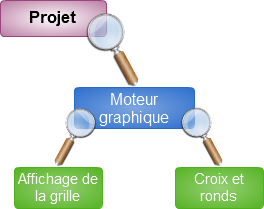
\includegraphics[scale=0.6]{images/slide1.png}
	% Une première approche : découper son projet au feeling en plus petites
	% parties. En prenant l’exemple d’un morpion, on peut distinguer une IA,
	% un moteur de jeu, graphiques, etc. Et ensuite on redécoupe ces moteurs,
	% avec l’exemple du moteur graphique entre affichage de la grille et des
	% pions.
	% Problème : il faut déjà savoir comment marche un projet pour savoir à
	% peu près comment découper et où aller.

	% TODO: refaire le graphique en incluant l’exemple du morpion de manière
	% visuelle.
  \end{center}
\end{frame}

\begin{frame}
  \begin{center}
    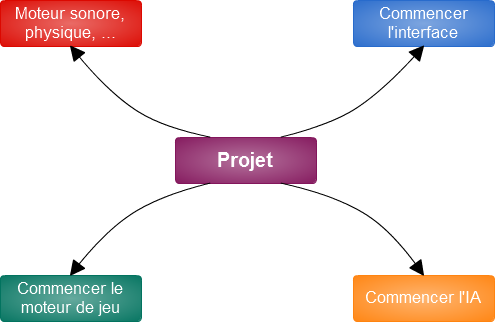
\includegraphics[scale=0.5]{images/slide2.png}
	% Découper le projet entre ce que chacun a envie de faire et chacun le
	% fait dans son coin. Quand on veut tout raccorder, à l’approche de la
	% soutenance, alors c’est l’emmerde. Va falloir réécrirer du code et
	% repenser pour interfacer son code avec celui des autres.
  \end{center}
\end{frame}

\begin{frame}
  \begin{block}{Un mix des deux}
    \begin{itemize}
      \item On découpe un maximum en réfléchissant avant de coder,
      \item chacun prend une partie et sait à peu près où il va,
      \item on reste dynamique.
    \end{itemize}
	% Meilleure méthode : essayer de penser avant de se mettre à coder à
	% l’architecture du projet. Définir les parties importantes, les
	% subdiviser et donner les parties les plus importantes au(x) plus
	% fort(s) ou selon les envies des gens.
	% Faire une base très solide et stable, sinon ça va être bancal, et au fur
	% et à  mesure des soutenances ça va devenir de pire en pire.
	% Essayer de se regrouper par paire : (un bon, un moins bon), le bon peut
	% travailler sur les parties les plus avancées et le moins bon peut
	% toujours demander de l’aide. Les deux connaissent bien leur partie.
  \end{block}
\end{frame}
